\section{Datasets for Sound Event Detection}
In order to evaluate the proposed method in polyphonic real-life conditions, we used the TUT Sound Events 2016 \& 2017 datasets, which were included in the corresponding editions of the DCASE Challenge. For the monophonic-SED case study, we used the TUT Rare Sound Events 2017 which represents the task 2 of the DCASE 2017 Challenge.

\subsubsection{TUT Sound Events 2016}
The TUT Sound events 2016 (TUT-SED 2016)\footnote{\url{http://www.cs.tut.fi/sgn/arg/dcase2016/}} dataset consists of recordings from two acoustic scenes, respectively ``Home'' (indoor) and ``Residential area'' (outdoor) which we considered as two separate subsets. These acoustic scenes were selected from the challenge organizers to represent common environments of interest in applications for safety and surveillance (outside home) and human activity monitoring or home surveillance \cite{mesaros2016tut}.
%The dataset was collected in Finland by Tampere University of Technology from different locations by means of a binaural recording system. For each location, a 3-5 minute long binaural
%audio recording is provided for a total of around 54 and 59 minutes of audio respectively for ``Home'' and ``Residential area'' scenario.
A total amount of around 54 and 59 minutes of audio are provided respectively for ``Home'' and ``Residential area'' scenarios.
Sound events present in each recording were manually annotated without any further cross-verification, due to the high level of subjectivity inherent to the problem. 
For the ``Home'' scenario a total of 11 classes were defined, % (including Object impact, People walking, Washing dishes),
while for the ``Residential Area'' scenario 7 classes were annotated. % (including Bird singing, Car passing by, People speaking).

Each scenario of the TUT-SED 2016 has been divided into two subsets: development dataset and evaluation dataset. The split was done based on the number of examples available for each sound event class. In addition, for the development dataset a cross-validation setup is provided in order to easily compare the results of different approaches on this dataset. The setup consists of 4 folds, so that each recording is used exactly once as test data. In detail, ``Residential area'' sound events data consists of 5 recordings in the evaluation set and 12 recordings in the development set while ``Home'' sound events data consists of 5
recordings in the evaluation set and 10 recordings in turn divided into 4 folds as training and validation subsets.


\subsubsection{TUT Sound Events 2017}
The TUT Sound Events 2017 (TUT-SED 2017)\footnote{\label{note_dcase17}\url{http://www.cs.tut.fi/sgn/arg/dcase2017/}} dataset consists of recordings of street acoustic scenes with various levels of traffic and other activities, for a total of 121 minutes of audio. The scene was selected as representing an environment of interest for detection of sound events related to human activities and hazard situations. It is a subset of the TUT Acoustic scenes 2016 dataset \cite{mesaros2016tut}, from which also TUT-SED 2016 dataset was taken. Thus, the recording setup, the annotation procedure, the dataset splitting, and the cross-validation setup is the same described above. The 6 target sound event classes were selected to represent common sounds related to human presence and traffic, and they include brakes squeaking, car, children, large vehicle, people speaking, people walking. The evaluation set of the TUT-SED 2017 consists of 29 minutes of audio, whereas the development set is composed of 92 minutes of audio which are employed in the cross-validation procedure.

\subsubsection{TUT Rare Sound Events 2017} 
The TUT Rare Sound Events 2017 (TUT-Rare 2017)\textsuperscript{\ref{note_dcase17}} \cite{DCASE2017challenge} consists of isolated sounds of three different target event classes (respectively, baby crying, glass breaking and gunshot) and 30-second long recordings of everyday acoustic scenes to serve as background, such as park, home, street, cafe, train, etc. \cite{mesaros2016tut}. In this case we consider a \textit{monophonic}-SED, since the sound events are artificially mixed with the background sequences without overlap. In addition, the event potentially present in each test file is known a-priori thus it is possible to train different models, each one specialized for a sound event. In the development set, we used a number of sequences equal to 750, 750 and 1250 for training respectively of the baby cry, glass-break and gunshot models, while we used 100 sequences as validation set and 500 sequences as test set for all of them. In the evaluation set, the training and test sequences of the development set are combined into a single training set, while the validation set is the same used in the Development dataset. The system is evaluated against an ``unseen'' set of 1500 samples (500 for each target class) with a sound event presence probability for each class equal to 0.5.

\subsection{Snore Sound Detection in Real Life Audio}
\label{ssec:dataset}
The snore detection algorithm has been evaluated on the A3-Snore dataset. A brief description of the acquisition setup and dataset splitting is provided in the following.

\subsubsection{Acquisition setup:}
In order to capture the overnight audio recordings a ZOOM-H1 Handy Recorder has been used. It is equipped with two unidirectional microphones set at a 90 degree angle relative to one another. The signals are stored in WAV files with a sampling rate of 44.1\ kHz and bit depth equal to 16.
The input gain is automatically set by the recorder to prevent overload and distortion, while the high-pass filter was enabled in order to eliminate pops, wind noise, blowing, and other kinds of low frequency rumble.


\subsubsection{Acquisition environment:}
The acquisition environment consist of a simple bedroom, with two access points (door and window). The recorder is placed near the patient, at same height of the bed and in line with the subject's mouth. During the recordings, the patient is the only one that can occupy the bedroom, in order to avoid contaminations on recorded audio signals. The room dimensions are reported in \figref{fig:room}.
Background sounds include traffic noise, breathing and speech signals, house and animal noises. We acquired some samples measurements of the event-to-background (EBR) ratios considering background noise, snoring events and noise events such as ``car passing by'' or ``dog barfing''. The EBR resulted equal to 6.5 dB and 1.1 dB respectively for noise to background EBR and snore to background EBR. 


\begin{figure}[t]
	\centering
	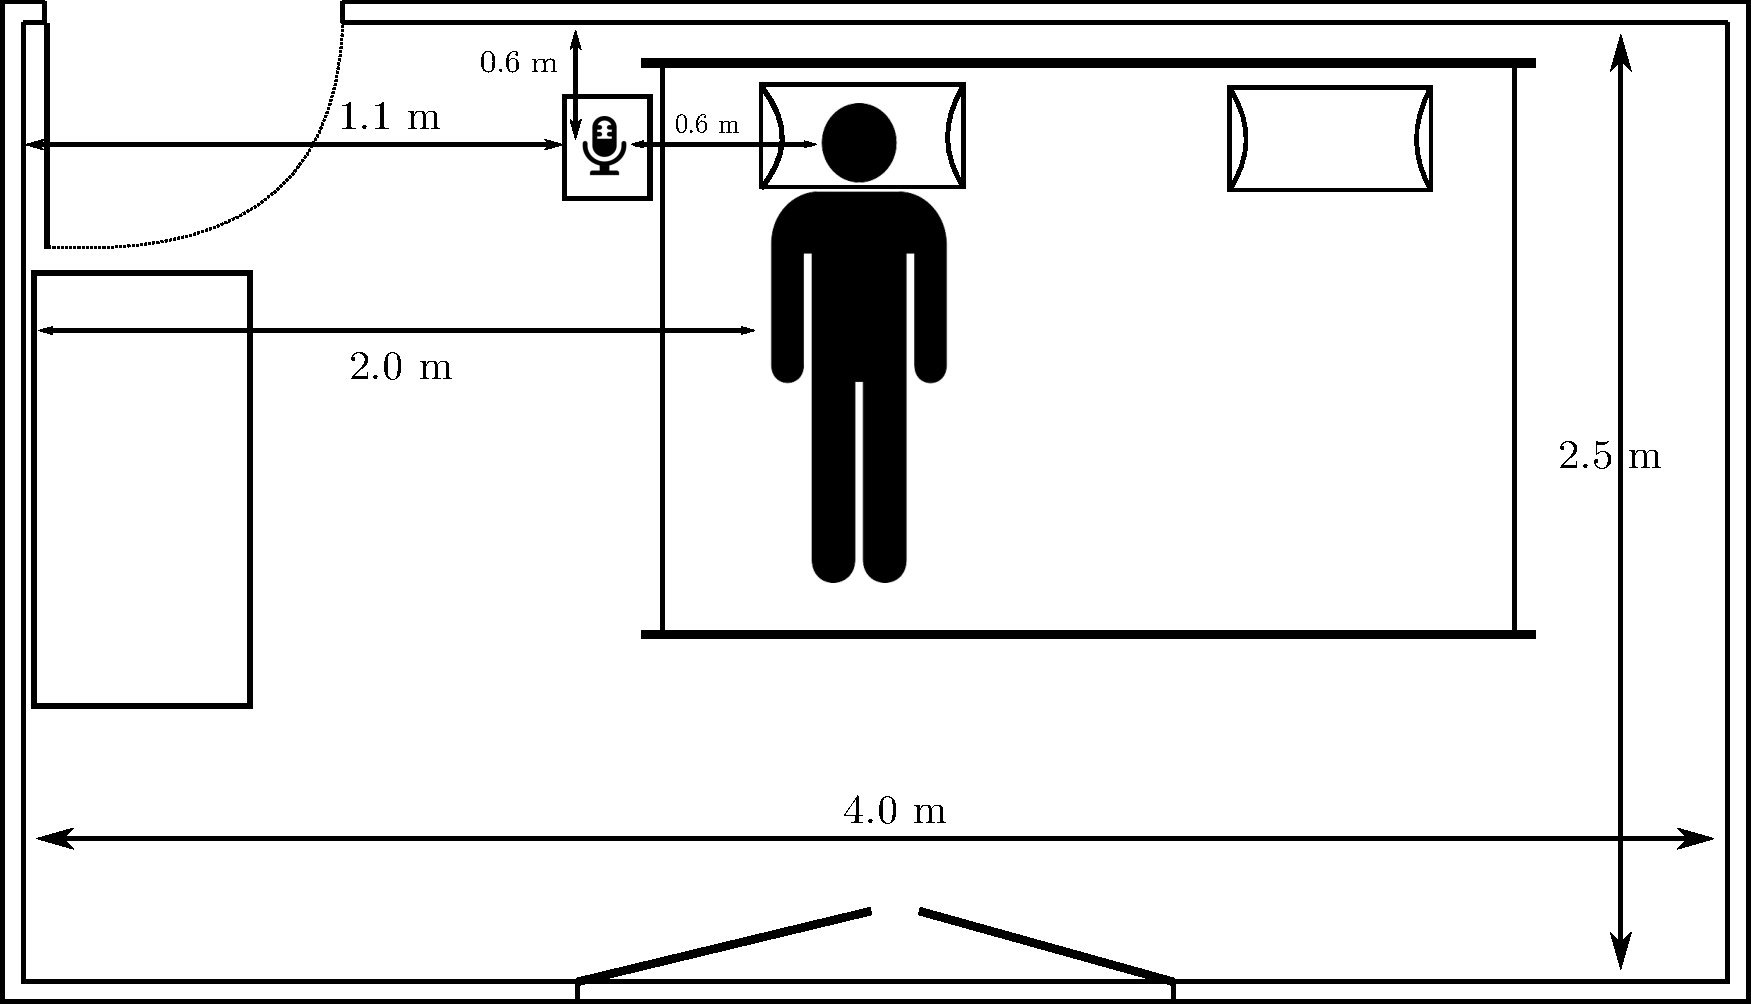
\includegraphics[width=0.8\columnwidth]{img/room.pdf}
	\caption{Plant of the recording room.} 
	\label{fig:room}
\end{figure}


\subsubsection{Dataset splitting:}
The original recordings have been manually labelled, annotating the snore events onset and offset with a resolution of 1 second. The audio sequences have been divided into chunks of 10 minutes, and only those with the highest number of snore events have been used in the experiments. 
The dataset is organized into subjects, which can be respectively used as \emph{training} or \emph{validation} sets in a two fold cross validation strategy (i.e., Leave One Subject Out procedure). The number of events per class in the database is strongly unbalanced as reported in \tableref{a3snore}. Thus, the snore detection task is challenging, due to the high number of noises on the A3-SNORE dataset. 

\begin{table}[ht]
	\centering
	\caption[A3-SNORE dataset]{Difference of recording times for each class, divided by snorers.}
	\begin{tabular}{cccccc}
		\hline
		\multicolumn{6}{c}{\textbf{A3-SNORE dataset}} \\
		\hline
		\# & Gender & Age & Snoring (SN) & Total Duration (Tot) & Ratio (SN/Tot) \\
		\hline
		Snorer 1 & M & 48 & 33m-27s & 3h-12m-0s & 14.5\% \\
		Snorer 2 & M & 55 & 21m-21s & 3h-50m-0s & 11.1\% \\
		\hline
		\multicolumn{3}{l}{Total} &	54m-48s	& 7h-02m-0s	& 12.8\%\\
		\hline    
	\end{tabular}	
	\label{a3snore} 
\end{table}

\subsection{Acoustic Novelty Detection}

\label{sec:databases}
This section describes the three databases evaluated in our experiments: A3Novelty, PASCAL CHiME, and PROMETHEUS.

\subsubsection{A3NOVELTY}

%FABIO Description of A3Corpus taken from ESWA paper. Io l'ho parafrasata in modo "light"...vedete voi se bisogna modificarla di più.

%TODO: add description of the database.

%TODO: add final table including stats on the datasets (number of abnormal sounds, duration etc...


The A3Novelty corpus\footnote{\label{note:a3}\url{http://www.a3lab.dii.univpm.it/research/a3novelty}} includes around 56 hours of recording acquired in a laboratory of the Università Politecnica delle Marche. 
These recordings were performed during different day and night hours, so very different acoustic conditions are available.
A variety of \emph{novel} events were randomly played back by a speaker (e.g., scream, fall, alarm or breakage of objects) during the recordings.

Eight microphones were used in the recording room for the acquisitions: four Behringer B-5 microphones with cardioid pattern and an
array of four AKG C400 BL microphones spaced by 4\,cm, then A MOTU 8pre sound card and the NU-Tech software were utilised 
to record the microphone signals. The sampling rate was equal to 48\,kHz.


The abnormal event sounds (cf.  Table \ref{tab:events}) can be grouped into four categories and they are freely available to download from \url{http://www.freesound.org}:
\begin{itemize}
	\item \textit{Sirens}, three different types of sirens or alarm sounds.
	\item \textit{Falls}, two occurrences of a person or an object falling to the ground.
	\item \textit{Breakage of objects}, noise produced by the breakage of an object after the impact with the ground.
	\item \textit{Screams}, four different human screams, both produced by a single person or by a group of people.
\end{itemize}


The A3Novelty corpus is composed of two types of recordings:
\emph{background}, which contains only background sounds such as human speech, technical tools noise and environmental sounds and \emph{background with novelty}, which contains in addition to the background the artificially generated novelty events.

In the original A3Novelty database the recordings are segmented in sequences of 30 seconds. In order to limit the size of training data, we randomly selected 300 sequences from the \emph{background} partition to compose of training material (150 minutes), and 180 sequences from the \emph{background with novelty} partition to compose the testing set (90 minutes). The test set contains 13 novelty occurrences.

For reproducibility, the list of randomly selected recordings, as well as the train and test set are made available % \footnotemark[\ref{note:a3}]. %ndFAB\footnotemark [3].


%\begin{table}[t]
%\centering
%\begin{tabular}{lccc}
%\hline
%\textbf{Rec Type} & \textbf{Day/Night} & \textbf{Length (hh:mm)} & \textbf{Novelty events}\\
%\hline
%\multirow{2}{*}{Background} & Day & 12:00 & -\\
%& Night & 24:00 & -\\
%\hline
%Background & Day & 9:00 & 16\\
%with novelty & Night & 12:00 & 30\\
%\hline
%\end{tabular}
%\caption{Recordings details.}
%\label{tab:recs_detail}
%\end{table}


\subsubsection{PASCAL CHiME}
\label{subsec:pascal}

The original dataset is composed of around 7 hours of recordings of a home environment, taken from the PASCAL CHiME speech separation and recognition challenge \cite{barker2013pascal}. 
It consists of a typical in-home scenario (a living room), recorded during different days and times,
while the inhabitants (two adults and two children) perform common actions, such as talking, watching television, playing, or eating. The dataset was recorded in stereo (with a binaural microphone) and a sample-rate of 16\,kHz. In the original PASCAL CHiME database the recordings are segmented in sequences of 5 minutes duration. In order to limit the size of training data, we randomly selected sequences to compose 100 minutes of background for the training set, and around 70 minutes for the testing set. For reproducibility, the list of randomly selected recordings, as well as the train and test set are made available\footnote{\url{http://a3lab.dii.univpm.it/webdav/audio/Novelty_Detection_Dataset.tar.gz}}. 
%The test set was generated adding different kinds of sounds\footnote{taken from www.freesound.org}, such as screams, alarms, falls and fractures (cf.\ Table \ref{tab:events}). 
%The test set did not include any overlapping events, the events were  and they were added at random position thus the distance between one event and another is not fixed. %ndFAB\footnotemark [1].
% %VES
The test set was generated adding different typologies of sounds\footnote{taken from www.freesound.org}, such as screams, alarms, falls and fractures (cf.\ Table \ref{tab:events}), after their normalization to the volume of the background recordings. % %
The events in the test set were added at random position (avoiding overlapping), thus the distance between one event and another is not fixed. %ndFAB\footnotemark [1].




\subsubsection{PROMETHEUS}
\begin{table}[t]
	\centering
	\tabcolsep=0.10cm
	\renewcommand{\arraystretch}{1.0}
	\caption[Acoustic novel events]{Acoustic novel events in the test set. Shown are the number of different events per database, the average duration, and the total duration in seconds per event type. The last column indicates the total number of events and total duration across the databases. The last line indicates the total duration in seconds of the test set including normal and novel events per database.}
	
	\begin{tabular}{ l || c c || c c || c c | c c | c c | c c || c c }
		\textbf{Events} & \multicolumn{2}{|c||}{A3Novelty} & \multicolumn{2}{|c||}{PASCAL CHiME} & \multicolumn{8}{|c||}{PROMETHEUS} & \multicolumn{2}{|c}{Total}\\
		\textbf{} & \multicolumn{2}{|c||}{} & \multicolumn{2}{|c||}{} & \multicolumn{2}{|c|}{ATM} & \multicolumn{2}{|c|}{Corridor} & \multicolumn{2}{|c|}{Outdoor} & \multicolumn{2}{|c||}{Smart-room} & \multicolumn{2}{|c}{}\\
		\textbf{} & \# & time(avg.) & \# & time(avg.) & \# & time(avg.) & \# & time(avg.) & \# & time(avg.) & \# & time(avg.) & \# & time\\
		\hline
		Alarm			& - & -		& 76 & 435.8 (6.0) 	 				& - & -			& 6 & 84.0 (14.0)	& - & -				& 3 & 9.0 (3.0)		& 85 & 528.8\\
		Anger			& - & - 				& - & - 				& - & -			& - & -				& 6 & 293.0 (48.8)		& - & - 			& 6 & 293.0\\  
		Fall 			& 3 & 4.2 (2.1)		& 48 & 89.5 (1.8) 	& - & -	 		& 3 & 3.0 (1.0)		& - & -				& 2 & 2.0 (1.0) 		& 55 & 98.7\\
		Fracture		& 1 & 2.2 			& 32 & 70.4 (2.2) 	& - & - 			& - & -				& - & -				& - & - 				& 33 & 72.6\\
		Pain			& - & -			 	& - & - 			& - & -	 		& 2 & 8.0 (4.0)		& - & -				& 5 & 67.0 (13.4) 		& 7 & 75.0\\
		Scream			& 6 & 10.4(1.7)		& 111 & 214.6 (1.9) 	& 5 & 30.0 (6.0)	& 25 & 228.0 (9.1)	& 4 & 48.0 (12.0)		& 10 & 234.0 (23.4) & 159 & 762.2\\
		Siren			& 3 & 20.4 (6.8)		& - & - 				& - & - 			& - & -				& - & -				& - & -				& 3 & 18.1\\
		\hline
		Total			& 13 & 38.1 (2.9) & 267 & 810.3 (3.1) 	& 5 & 30.0 (5.0) 		& 36 & 323.0 (9.0) 	& 10 & 341.0 (34.1) 	& 20 & 312.0 (15.6) & 348 & 1848.4\\
		\hline\hline
		Test time & - & 5400.0 				& - & 4188.0 	& - & 750.0			& - & 960.0	& - & 1620.0				& - & 1020.0		& - & 13938.0\\
		
	\end{tabular}
	\label{tab:events}
\end{table}

The PROMETHEUS database \cite{ntalampiras:probabilistic} contains recordings of various scenarios designed to serve a wide range of real-world applications. The database includes: 1) a \textit{smart-room} indoor home environment including phases where a user is interacting with an automated speech-driven home assistant, 2) an outdoor public space consisting of \textit{a}) interaction of people with an \textit{ATM}, \textit{b}) an \textit{outdoor} security scenario in which people are waiting in front of a counter, and 3) an  indoor office \textit{corridor} scenario for security monitoring in standard indoor space. 
%The first one is intended to be representative of particular activities which take place inside an intelligent environment, including phases where the user is interacting with an automated speech-driven home assistant. As for the second setting, two scenarios with different scopes were captured: 1) ATM scenario, which included interactions of people with an ATM, and 2) security scenario, in which people in a queue are waiting for service in front of a counter and can be utilized as a general-purpose scenario with many applications (e.g., bank, airport, etc.). The third setting was used for security scenarios in a standard indoors space. 
These scenarios substantially differ in terms of acoustic environment. The indoor scenarios were recorded under quiet acoustic conditions, whereas the outdoor recordings were conducted in an open-air public area and contain non-stationary background noise.   
The smart-home scenario contains recordings of five professional actors performing five single-person and 14 multiple-person action scripts. The main activities include human-machine interaction with a virtual home agent, a number of alternating normal and abnormal activities specifically designed to monitor and interpret human behaviour. The single-person and multiple-person actions include abnormal events, such as: falls, alarm followed by panic, atypical vocalic reactions (pain, fear, anger), or fractures. Examples are: walking to the couch, sitting or interacting with the smart environment to turn the TV on, open the windows, or decrease the temperature. The scenarios were recorded three to five times, by changing the actors and their roles in the action scripts.
Table \ref{tab:events} provides details on the number of abnormal events per scenario, including average time duration.


\section{The DIRHA Dataset}
\label{sec:dataset}

\begin{figure}[h]
	\centering
	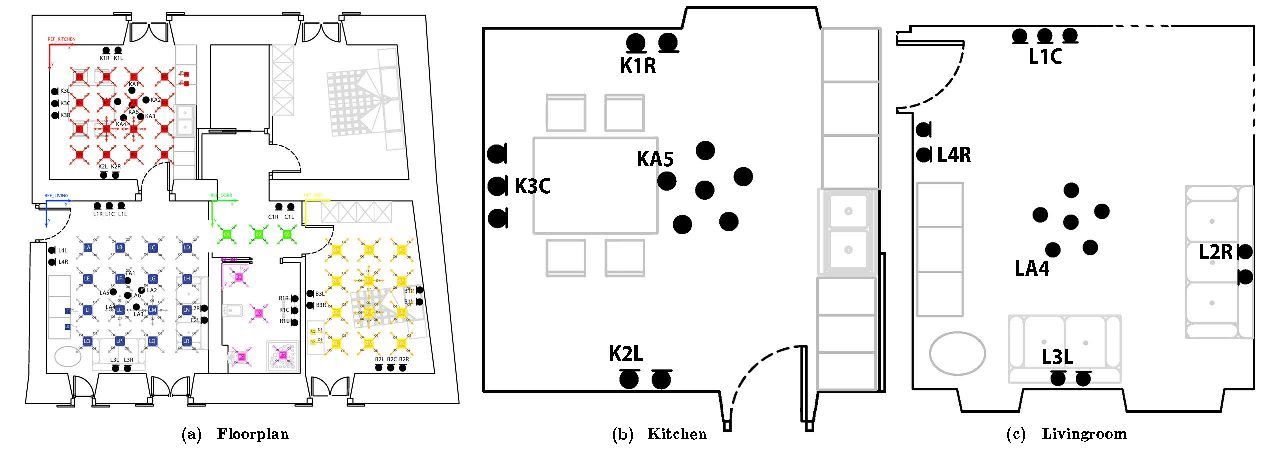
\includegraphics[width=\textwidth]{img/plan}
	\caption{The map of the apartment used for the DIRHA project (a). Figures (b) and (c) show the considered rooms, with the disposition of their relative microphones. }
	\label{fig:DIRHA_map}
\end{figure}

The analysis of the DNN-SLOC performance has been conducted on the DIRHA dataset \cite{cristoforetti2014dirha}, characterized by diverse scenes, rooms, microphones and noise conditions\footnote{\url{http://dirha.fbk.eu/simcorpora}}. In details, the apartment where the dataset has been recorded consists in five rooms and a total of 40 microphones. These are arranged in linear and circular arrays, with the first ones placed on the walls of all rooms, and the circular ones are placed on the ceiling of the living room and of the kitchen (\figref{fig:DIRHA_map}).

The dataset is composed of two subsets, named \emph{Simulated} and \emph{Real}. For each of them several \textit{scenes} have been recorded, composed of typical situations observable in a domestic context. As reported in \tableref{tab:dataset}, the two subsets differ in terms of scenes and total length: in the Simulated set the scenes length is fixed to 60 seconds, while it varies in the Real set. In addition, the latter has been recorded with persons moving in the rooms and speaking towards different directions throughout the scenes, whilst the Simulated has been obtained by convolving a fixed set of measured Room Impulse Responses (RIRs) with recorded signals.
The Simulated subset is also characterized by a lower SNR compared to the Real one and overlapping speech does not occur.

Our study focuses on two rooms of the dataset, i.e.,  the Kitchen and the Living Room, due to three main aspects. First of all, these rooms consist in the area of a home-environment where most of the events take place. In addition, being the widest rooms of the apartment, the localization task is more challenging. \textcolor{red}{The room dimensions are respectively $4.79$\,m~$\times$~$3.80$\,m for the Kitchen and $4.79$\,m~$\times$~$4.85$\,m for the Living Room.}
Finally, the number of microphones are higher compared to the other rooms, and they comprise both wall and ceiling arrays.

\begin{table}[t]
	%\renewcommand{\arraystretch}{1.2}
	\centering
	%	\small
	\caption{Main differences between the Real and Simulated subsets.}
	\resizebox{.75\columnwidth}{!}{%
		\begin{tabular}{c|c|c}\hline
			& \textbf{Real} & \textbf{Simulated} \\ \hline
			\textbf{Nr.\ of Scenes}  & 22 & 80 \\ \hline
			
			\textbf{Total Duration} &  21.5 min. & 80 min.  \\  \hline
			\multirow{2}{*}{\textbf{Speech Percentage}}	&  12.9\%  & 23.6\%  \\
			& 	2.8  min.	& 18.9 min. \\ \hline
			\textbf{Source} & human (moving) & loudspeaker (static) \\ \hline
			\textbf{Background} & quiet & various \\ \hline
			\textbf{Noise Source Rate} & low & high \\ \hline
			\textbf{Overlapping Events} & no & yes \\ \hline  
		\end{tabular} 
	}
	\label{tab:dataset}
\end{table}